\documentclass{cls/iutbscthesis}
\usepackage{kantlipsum} % This package is used to generate place holder text. Remove it in the actual world. 

% The iutbscthesis uses biblatex for bibliography management.
% You can learn the basics of biblatex from:
% https://www.overleaf.com/learn/latex/Bibliography_management_with_biblatex

\ExecuteBibliographyOptions{
  sorting=none,       % Sort by order of appearance
}

\addbibresource{citations.bib}

% The complete title of your thesis, mandatory
\title{Multi-Organ and Tumor Segmentation by Context-Aware Attention with BioBERT and Global Spatial Reasoning}

% Use the \addauthor command to keep adding authors with student ID
\addauthor{Mirza Mohammad Azwad}{200042121}
\addauthor{Rhidwan Rashid}{200042149}
\addauthor{M M Nazmul Hossain}{200042118}

% Use the \supervisor command to define the supervisor with name, designation, and department
% There needs to be one and only one supervisor
\supervisor{Tareque Mohmud Chowdhury}{Assistant Professor}{Department of Computer Science and Engineering}
\addcosupervisor{Farzana Tabassum}{Lecturer}{Department of Computer Science and Engineering}

% % Use the \addcosupervisor command to add a cosupervisor. There might be no cosupervisor at all
% % In that case, just remove all of the \addcosupervisor commands.
% \addcosupervisor{Dr.\ Sue Permann}{Assistant Professor}{Department of Computer Science and Engineering}
% \addcosupervisor{Mr. Francis FullOfFrenchPeople}{Lecturer}{Department of Computer Science and Engineering}

% Complete department name, mandatory
\department{Department of Computer Science and Engineering}

% Complete program name, mandatory
\program{BACHELOR OF SCIENCE IN COMPUTER SCIENCE AND ENGINEERING}

% Date (day, month name, and year) when the presentation took place, mandatory
\defensedate{27}{April}{2025}

\begin{document}

%-------------------------- FRONT MATTER --------------------------%

% Generate cover page of the report to be printed on the hard cover
\coverpage

% Switch to roman page numbering
\pagenumbering{roman}

% Generate the title leaf, mandatory
\titlepage

% Auto generate declaration of candidate based on previous info, mandatory
\declarationofcandidate

% Dedicate report to someone. You may add more sentences to it.
\dedicatedto{our supervisor, whose guidance and support made this research journey smooth and successful.}

\tableofcontents
\listoffigures

\clearpage

% Add abbreviations within this environment using the \abbr command
\begin{abbreviations}
    \abbr{CT}{Computed Tomography}
    \abbr{MRI}{Magnetic Resonance Imaging}
    \abbr{CNN}{Convolutional Neural Network}
    \abbr{nnU-net}{Not a New U-net}
    \abbr{DoDNet}{Dynamic On Demand Network}
    \abbr{FUSE}{Fusion and Selection}
    \abbr{BraTS}{Brain Tumor Segmentation}
    \abbr{MOTS}{Multi Organ Tumor Segmentation}
\end{abbreviations}

% Any acknowledgement that you want to write goes in the following environment
\begin{acknowledgement}

We would like to express our deepest gratitude to our supervisor, Mr.\ Tareque Mohmud Chowdhury, and our co-supervisor, Ms.\ Farzana Tabassum, Lecturer, Bioinformatics Lab, Department of Computer Science and Engineering, Islamic University of Technology, for their continuous guidance, valuable feedback, and unwavering support throughout the course of this project. Their expertise and encouragement have been instrumental in shaping our work.

We also wish to extend our sincere thanks to the Department of Computer Science and Engineering at Islamic University of Technology for providing us with the necessary resources and an inspiring academic environment.

\end{acknowledgement}


% Write your abstract here.
\begin{abstract}
Accurate segmentation of multiple organs and tumors in medical images is critical for enhancing clinical workflows, yet existing methods often struggle with capturing long-range spatial dependencies, leveraging domain-specific semantics, and generalizing across diverse imaging modalities. This thesis addresses these challenges by proposing a novel hybrid architecture that integrates context-aware attention mechanisms with biomedical semantic embeddings to achieve robust multi-organ and tumor segmentation.  

The proposed framework combines a CNN-Transformer hybrid encoder for local and global feature extraction, a \textit{BioBERT}-enhanced universal prompt module to infuse domain-specific knowledge, and a \textit{FUSE} prompt decoder for task-aware feature fusion. By incorporating \textit{BioBERT}---a biomedical language model---the model enriches task prompts with anatomical and clinical semantics, enabling better understanding of organ-tumor relationships. The \textit{TransAttUNet}-inspired encoder-decoder backbone, augmented with multi-scale skip connections, ensures precise reconstruction of segmentation masks while addressing spatial complexity.  

Three diverse datasets: \textit{MOTS} (abdominal CT), \textit{BraTS 2021} (brain MRI), and \textit{Prostate MRI}---are utilized to evaluate the model's performance across modalities and anatomical regions. These datasets present unique challenges, including interclass imbalance, multimodal data integration, and low-context scenarios, providing a comprehensive testbed for assessing generalization capabilities.  
\end{abstract}

%-------------------------- MAIN BODY --------------------------%
% Switch to arabic page numbering
\pagenumbering{arabic}

\chapter{Introduction}
Medical image segmentation is the process of identifying and delineating anatomical structures or regions of interest (such as organs, tissues, or lesions) within biomedical images. In clinical diagnosis and planning, segmentation serves to “delineate the objects of interest from the complex background on various biomedical images”\cite{chen2024transattunet}. A special case of this is multi-organ segmentation, where multiple anatomical structures (and potentially associated pathological regions) are segmented simultaneously. For example, in cancer treatment planning one often needs both a tumor mass and its surrounding organs-at-risk (OARs) outlined in a scan\cite{liu2024multiorgan}. Similarly, tumor detection refers to identifying suspicious regions that correspond to tumors; when combined with segmentation, it provides precise boundaries of tumors for analysis and intervention. These tasks are highly relevant to healthcare. Accurate organ and tumor segmentation can greatly aid computer-aided diagnosis, surgical planning, and radiotherapy, improving treatment outcomes and patient safety\cite{liu2024multiorgan}. Thanks to advances in artificial intelligence and deep learning, fully automated segmentation methods have dramatically improved in recent years. In fact, modern deep learning–based segmentation models now “far outperforms traditional methods” and have become a major research topic\cite{liu2024multiorgan}. This has paved the way for integrating AI tools into clinical workflows, helping to reduce manual workload and inter-observer variability.

\section{Motivations and Scope}
% In this section, you should explain why your research matters. Begin by reflecting on what motivated you to tackle this particular problem. Personal experiences or global challenges might have inspired your interest. For example, perhaps you're driven by the potential societal impact of your work, or maybe the research addresses a critical gap in your field. This is where you connect your personal motivations with the broader implications of your study. Following this, provide a succinct review of key research that has informed your understanding of the topic. Keep this review brief—just enough to show how previous studies have contributed to your thinking—since you'll explore related works in more depth in the next chapter. Finally, highlight the limitations or gaps in current knowledge that your thesis seeks to address. By identifying these voids, you build a compelling case for why your research is necessary.
The motivation for this research arises from the need of accurate, efficient, and reliable segmentation of organs and tumors in medical images. For example, in radiation therapy for cancer, precise delineation of tumor volumes and nearby normal organs is essential to target tumor tissue while sparing healthy tissue.\\

Currently, segmentation is often performed manually by clinicians, which is time-consuming (e.g., contouring 24 organs in head-and-neck CT can take over 3 hours, labor-intensive, and subject to differences. Also, a shortage of trained experts can lead to delays in treatment and inconsistent results.
Automated segmentation promises to ease this process, enabling faster treatment planning and more standardized outcomes.\\

Despite many progresses, existing segmentation models have limitations that motivate further research. Zhang et al. proposed a Dynamic On-demand Network (DoDNet) that tackles partially labeled multi-organ data by using task-conditioned filters and a dynamic head\cite{zhang2021dodnet}. On the other hand, Liu et al. introduced a CLIP-Driven Universal Model that uses text embeddings from a vision-language model (CLIP) to encode anatomical relationships, enabling segmentation of 25 organs and 6 tumor types\cite{liu2023clip}. However, because CLIP is pretrained on natural images, its medical generalization is limited.\\

Deep learning approaches like U-Net and its variants have achieved significant performance, but they usually focus on individual organs or single imaging modalities. For example, the nnU-Net framework (a self-configuring U-Net) has set high benchmarks across diverse medical segmentation challenges \cite{isensee2021nnunet}, but it relies only on convolutional operations and local context. Such CNN-based models may struggle to capture long-range spatial relationships, which can be important when organs or tumors span large/very small regions of the image. Recent transformer-augmented networks (such as TransAttUNet\cite{chen2024transattunet}) attempts to address this by adding attention modules, but these models can be computationally heavy and still may not fully leverage prior anatomical knowledge.\\

These observations reveal gaps in the current literature. Existing approaches tend to be specialized (focusing on one organ or modality) or require task labels that ignore rich anatomical relationships. There is no unified framework that both captures global image context and incorporates domain-specific knowledge for segmentation. In this thesis, we aim to address these gaps by developing methods that bridge CNN and transformer techniques, leverage multi-modal data, and integrate biomedical semantics into the segmentation process.

\section{Problem Statement}
% The problem statement is the core of your thesis. It should be a concise, clear statement that encapsulates the issue your research is tackling. Following this, list two to four specific research objectives. These objectives will guide the structure of your work and must align closely with the problem you are addressing. These are not just high-level goals—they will shape how you approach the research and structure your experiments, making them crucial to the development of your thesis.
Given a collection of $N$ datasets $\{D_1, D_2, \dots, D_N\}$, where each $D_i = \{(X_{ij}, Y_{ij})\}_{j=1}^{n_i}$ consists of $n_i$ medical images $X_{ij}$ and their corresponding ground truth segmentations $Y_{ij}$, the goal is to perform segmentation of multiple organs and tumors across diverse imaging modalities and anatomical regions.


\section{Research Challenges}
% Every field has its unique challenges, and this is the section where you should discuss those specific to your research domain. Avoid generic descriptions; instead, focus on the more nuanced difficulties your research aims to confront. For example, if you're working in machine learning, you might highlight the challenge of dealing with noisy data or balancing the trade-offs between algorithmic efficiency and accuracy. In language translation, the challenge might not simply be translating words but handling complex sentence structures, finding appropriate cultural or linguistic equivalents, or maintaining grammatical accuracy. Be sure to mention any unresolved challenges in your field that demand innovative solutions, particularly those your work seeks to address. This establishes the significance and difficulty of your project while showcasing the real obstacles that make your research exciting and valuable.
\begin{itemize}
    \item \textbf{Difficulty in capturing long-range spatial dependencies using CNN-based backbones like nnU-Net:} Classical convolutional architectures like U-Net and nnU-Net have small receptive fields and are based heavily on local information. While this is fine for small or confined anatomical structures, it is rather challenging if dealing with spatially extensive or complex regions (such as tumors that cross the boundaries of organs). The former is suboptimal for capturing long-range structure using these models without explicit architectural modifications.

    \item \textbf{Inability to leverage biomedical domain knowledge effectively in segmentation prompts:} Recent approaches leveraging vision-language models or prompt guided embeddings have unlocked new possibilities, but there is a catch: most of them rely on general-purpose models such as CLIP, which were not trained to understand medical concepts. Therefore, the anatomical and clinical semantics are not effectively represented with prompts, and segmentation models may not understand organ-tumor interactions or typical spatial arrangements.

    \item \textbf{High domain shift sensitivity when transferring models across datasets or imaging modalities:}
    A model which was trained on abdominal CT might perform poorly on brain MRI because of domain shifts in intensity distributions, resolution, organ appearance, and annotation protocols. This prevents generalization, and requires either domain-specific fine-tuning or robust architectures.

    \item \textbf{Limited interpretability in prompt-guided segmentation due to opaque fusion mechanisms: } Though prompts are used to guide segmentation in prompt-driven segmentations, it is often unclear how the prompts influence the outcome. The fusion mechanism in many existing models are treated as a black box, which makes it difficult to debug, refine, and understand the decision-making process. This lack of interpretability becomes a concern in clinical settings where transparency is crucial.
\end{itemize}
% Nazmul Bad dite bolse
% Azwad add korte bolse
% ...................
%CDI FALTU JINISH T^T
\section{Contribution}

This research proposes a novel hybrid segmentation pipeline that integrates a Transformer-based encoder (TransAttU-Net) \cite{chen2024transattunet}) with a BioBERT-driven prompt decoder.
\par
The key contributions of this research are summarized as follows:
\begin{itemize}
    \item \textbf{Development of a domain-aware universal segmentation framework} that bridges global spatial reasoning with biomedical semantic understanding.
    
    \item \textbf{Critical evaluation of state-of-the-art prompt-driven models:} Through a comparative analysis of existing universal segmentation models such as DoDNet~\cite{zhang2021dodnet}, CLIP-driven segmentation models~\cite{liu2023clip}, and UniSeg~\cite{ye2023uniseg}, several architectural shortcomings were identified. These include delayed prompt fusion, limited global spatial modeling, and inadequate semantic grounding using general-purpose embeddings.
\end{itemize}


\section{Organization}
% Finally, provide a brief roadmap of your thesis. This section helps orient your reader and ensures a logical flow of ideas throughout the document. Explain how each chapter is structured and how the various parts of your thesis fit together to form a coherent whole. This organizational overview ensures that readers can follow your arguments and see the connections between your objectives, methods, and conclusions, leading them through the narrative of your research from introduction to conclusion.
The rest of the thesis is organized as follows:
\begin{itemize}
    \item \textbf{Chapter 2: Related Works} In this chapter, we surveyed existing works on multi-organ tumor segmentation. It also includes traditional algorithms and deep learning methods. We mainly focused on recent architectures, such as U-Net variants, transformer based networks, prompt driven architectures etc. and discussed various approaches.
    
    \item \textbf{Chapter 3: Proposed Methodology} Here we presented our proposed pipeline. It includes out innovative pipeline for multi-organ tumor segmentation and describes it in detail.
    
    \item \textbf{Chapter 4: Results and Discussion} This chapter describes and and addresses the challenges of the datasets(MOTS, BraTS21, ProstateMRI) we are using for our thesis. It also includes insight in each dataset and their unique features.
    
    \item \textbf{Chapter 5: Conclusion} In this chapter, we summarize everything we have done until now restating the contributions and future directions of our thesis.
\end{itemize}

\chapter{Related Works}
During the last decade, with the increased novelty of deep learning architectures and the advent of attention mechanisms \cite{vaswaniAttention}, continuous efforts have been made to integrate deep learning architectures to create automated clinical workflows. Furthermore, advances in medical image segmentation have been pivotal for automating these clinical workflows with the goal of multi-organ and tumor detection. Since its inception, the research has evolved from task-specific models to universal frameworks capable of handling diverse organs and tumors across different image modalities, i.e., CT scans, MRI scans, PET scans, etc. In this section, we present a narrative that traces this evolution, highlighting the foundational architectures, dynamic models, prompt-driven segmentation, and their respective challenges and contributions. In Figure \ref{fig:taxonomy-and-chronology}, we showcase the evolution of the field and our focus area for this thesis work.
\begin{figure}[h!]
    \centering
    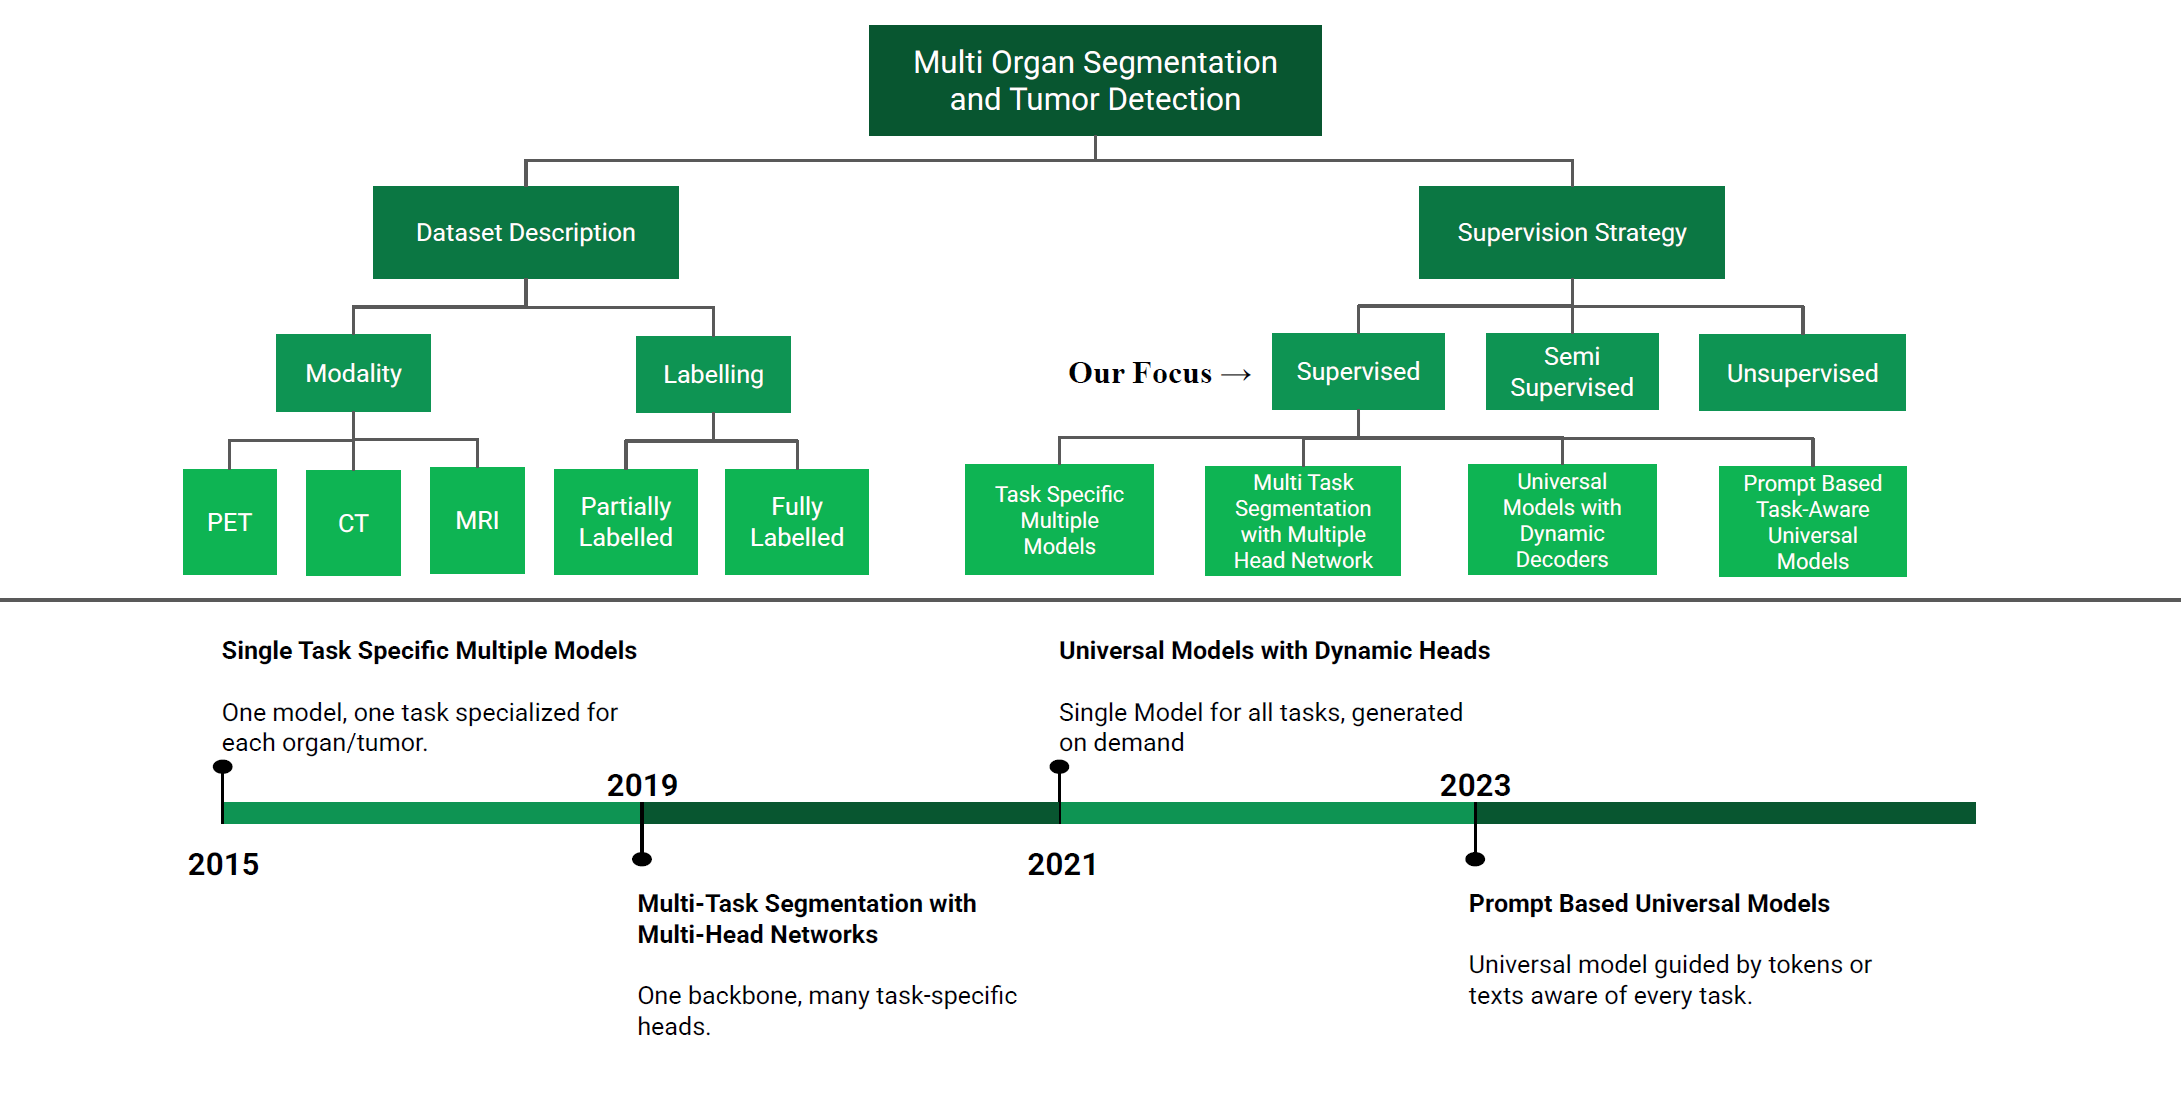
\includegraphics[width=1\linewidth]{figs/taxonomy.png}
    \caption{Evolution of Multi-Organ Tumor Segmentation and Our Focus Area in this particular domain}
    \label{fig:taxonomy-and-chronology}
\end{figure}

\section{Foundations}
The emergence of U-Net \cite{ronneberger2015unet} revolutionized biomedical image segmentation by introducing a contracting-expanding encoder-decoder architecture with skip-connections. U-Net's capability to produce dense per-pixel predictions even from a few annotated samples laid the groundwork for the first generation of medical segmentation deep learning networks.
\par
Standing on U-Net's shoulders, nnU-Net \cite{isensee2021nnunet} offered a self-configuring framework that automated hyperparameter tuning, cross-validation, network adaptation, and pre/post-processing, achieving strong performance across diverse biomedical datasets without requiring much manual intervention.
\par
However, these models were inherently designed for single tasks. Each new organ or tumor type would mean having to train a separate model, leading to scalability issues. Furthermore, convolutional architectures, while powerful, struggled to model long-range spatial dependencies critical for complex anatomical relationships. \cite{chen2024transattunet}
\par
To address these limitations, TransAttUNet~\cite{chen2024transattunet} introduced Transformer-based self-attention mechanisms into the U-Net structure, aiming to overcome the local receptive field constraints of standard convolutions. By incorporating both Transformer Self-Attention (TSA) modules and Global Spatial Attention (GSA) modules at the bottleneck of the encoder-decoder framework, TransAttUNet enabled the modeling of non-local dependencies and contextual interactions across the entire image space. Additionally, multi-scale skip connections aggregated semantic features at different resolutions, helping to recover fine anatomical details lost during downsampling. This combination of convolutional localization and Transformer-driven global reasoning significantly improved segmentation performance on complex medical imaging tasks, setting a new direction for hybrid CNN-Transformer architectures in biomedical segmentation.

\section{Addressing Complexity}
To improve scalability, researchers transitioned to multi-task segmentation networks such as Med3D \cite{chen2019med3d} and TAL-Net \cite{shang2024triaxial}. Med3D introduced the concept of sharing a common encoder across tasks while utilizing multiple task-specific decoders, enhancing data efficiency. Similarly, TAL-Net adopted adaptive loss functions to manage partially labeled data across multiple decoder heads.
\par
While it did make it easier to train over multiple tasks, these multi-head architectures incurred high inference costs and lacked flexibility: adding new tasks now requires architectural redesign and retraining. However, managing multiple active decoders simultaneously posed memory and computational challenges.

\section{Towards Universality}
Following the influence of multi-head systems, dynamic segmentation models soon began to come to the limelight. DoDnet \cite{zhang2021dodnet} first proposed a single encoder-decoder network with a dynamic head that changes on demand, in order to be conditioned on task-specific information. They also managed to encode each task as a one-hot vector and generated dynamic convolution kernels. In addition, Zhang et al. came up with the MOTS dataset by combining various other datasets. DoDNet also enabled training on multiple partially labeled datasets without architectural modifications.
\par
The dynamic approach marked a major shift by addressing the partial labeling issue prevalent in medical datasets. However, the reliance on one-hot encoding for the prompts ignored semantic relationships between tasks, i.e. the natural connection between liver and liver tumor, essentially any organ and its corresponding tumor. Additionally, introducing task-awareness only at the final decoding state limited the model's ability to handle complex anatomical targets effectively.

\section{Introducing Semantics}
To overcome the semantic limitations of one-hot encoding, language-vision models were introduced. The CLIP-Driven Universal Model \cite{liu2023clip} incorporates text embeddings served from CLIP to represent organs and tumors, capturing anatomical relationships. By using the semantic embeddings instead of rigid task vectors, the model improved generalization and allowed easy extensibility: new tasks could be added simply by providing new textual labels without retraining.
\par
Although performance heavily depended on the alignment between CLIP's pretraining and medical domain knowledge which was a lacking in case of CLIP.

\section{Early Task Awareness}
Building upon the works of Zhang et al. and Liu et al., UniSeg \cite{ye2023uniseg} introduced the novel prompt-driven segmentation paradigm. Instead of introducing task-specific conditioning at the decoder output, UniSeg injected learnable universal prompts early into the model pipeline through a FUSE module, allowing the encoder and decoder to co-train in a task aware manner from the beginning.
\par
The design allowed better modeling of inter-task relationships and improved feature representations across multiple modalities and domains. UniSeg outperformed earlier universal models like DoDNet \cite{zhang2021dodnet} and CLIP-driven frameworks \cite{liu2023clip}, demonstrating superior Dice scores on various organ and tumor segmentation benchmarks. Nonetheless, UniSeg's prompts were purely learnable without explicit biomedical domain grounding, leaving room for further improvements in semantic fidelity.

\section{Identified Gaps and Research Opportunities}
While significant progress has been made, several gaps persist:
\begin{itemize}
    \item \textbf{Long-Range Spatial Reasoning}: CNN-based backbones like U-Net and nnU-Net have limitations in modeling long-distance anatomical dependencies
    \item \textbf{Semantic Grounding}: Existing prompt-based models lack explicit incorporation of medical knowledge, relying on either learnable or general-purpose language embeddings
    \item \textbf{Cross-Domain Generalization}:  Domain shifts across modalities (e.g., CT vs MRI) still challenge universal models, as observed in generalization studies
    \item \textbf{Explainability}: Prompt-based fusion mechanisms remain opaque, hindering clinical trust and interoperability
\end{itemize}

These gaps motivate our proposed enhancements that aim to replace CNN-based encoders with Transformer-based architectures for better global spatial reasoning, and to enrich task prompts with biomedical semantics via models like BioBERT.

\section{Summary}
In summary, the trajectory of research in multi-organ segmentation and tumor detection has evolved from specialized task-specific models to dynamic universal frameworks, and further towards prompt-driven, semantically informed architectures. Each advancement has addressed critical limitations of its predecessors but introduced new challenges, particularly around semantic understanding and spatial reasoning. Our work builds on these insights to further enhance universality, and domain generalization in medical image segmentation.

\chapter{Proposed Methodology} \label{chapter:proposed}

\section{Introduction}

This chapter presents the detailed methodology developed to address the challenges in universal multi-organ and tumor segmentation. Building upon the strengths of convolutional feature extraction, global Transformer-based context modeling, and semantic prompt-driven guidance, the proposed hybrid framework introduces a BioBERT-enhanced FUSE module, integrated into a TransAttUNet-inspired encoder-decoder backbone. By merging fine-grained spatial features with long-range dependencies and biomedical task-specific knowledge, the architecture aims to deliver accurate and generalizable segmentation across diverse modalities.

\section{Overview of the Methodology}

The proposed system follows an encoder-decoder paradigm enriched with global self-attention, prompt-driven task conditioning, and multiscale feature fusion. Specifically, a CNN-Transformer hybrid encoder extracts hierarchical features from the input images. BioBERT embeddings, representing task semantics, are fused with visual features through an enhanced FUSE module to create task-specific prompts. These prompts interact with encoded visual tokens via a transformer decoder module inspired by DETR-like architectures. Finally, a CNN-based decoder reconstructs high-resolution segmentation maps, leveraging skip connections at multiple scales to preserve fine details.

Figure~\ref{fig:proposed_pipeline} illustrates the overall architecture.

\begin{figure}[h!]
    \centering
    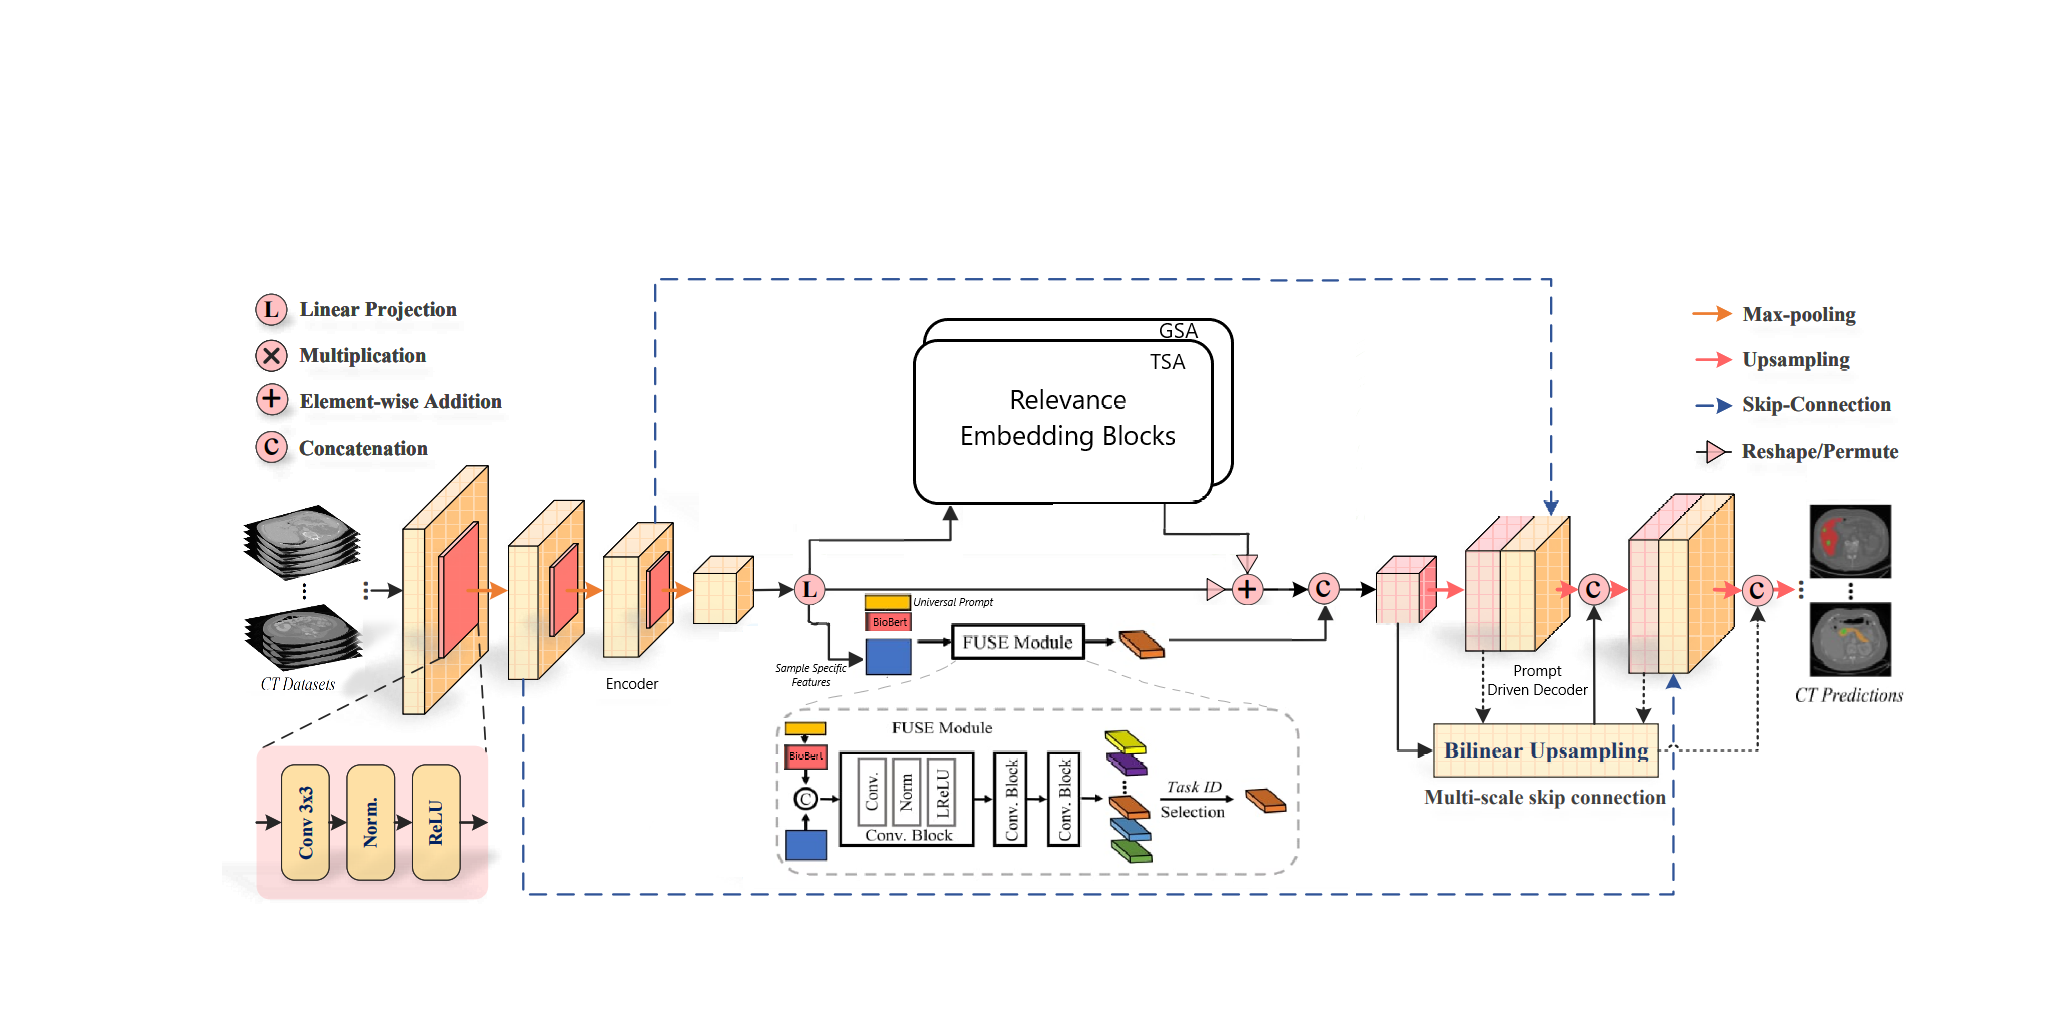
\includegraphics[width=\textwidth]{figs/proposed_pipeline2.png}
    \caption{Proposed Hybrid Architecture Integrating BioBERT-FUSE Prompting with TransAttUNet-style CNN-Transformer Backbone.}
    \label{fig:proposed_pipeline}
\end{figure}

\section{Chronological Breakdown of Components}

\subsection{Problem Formulation}

Given $N$ segmentation tasks $\{D_1, D_2, \ldots, D_N\}$ where $D_i = \{(X_{ij}, Y_{ij})\}_{j=1}^{n_i}$, with $X_{ij}$ representing input images and $Y_{ij}$ their corresponding ground truths, the objective is to learn a unified model $\mathcal{M}$ capable of segmenting all tasks with minimal performance degradation. Straightforward solutions involve training $N$ separate models; however, they ignore task correlations and impose significant redundancy~\cite{ye2023uniseg}.

\subsection{CNN-Transformer Hybrid Encoder}

The encoder integrates convolutional blocks for local feature extraction and Transformer blocks for modeling global context~\cite{ronneberger2015unet,vaswaniAttention}. 
Each input image $X \in \mathbb{R}^{C \times H \times W}$ passes through:
\begin{itemize}
    \item \textbf{Convolutional stages}: Multiple $3\times3$ convolutional layers, instance normalization, ReLU activations, and strided down-sampling.
    \item \textbf{Transformer stages}: Vision Transformer layers operating on flattened feature maps, incorporating Multi-Head Self-Attention (MHSA).
\end{itemize}

MHSA operation at each layer is defined as:
\begin{equation}
    \text{Attention}(Q, K, V) = \text{softmax}\left(\frac{QK^T}{\sqrt{d_k}}\right)V,
\end{equation}
where $Q$, $K$, $V$ are queries, keys, and values projected from the input features.
\par
Additionally, inspired by TransAttUNet~\cite{chen2024transattunet}, self-attention layers are enhanced with:
\par
\textbf{Transformer Self-Attention (TSA)}:
\begin{equation}
    TSA(Q, K, V) = \text{softmax}\left(\frac{QK^T}{\sqrt{d_k}}\right)V.
\end{equation}

\textbf{Global Spatial Attention (GSA)} mechanism aggregates features spatially to complement TSA:
\begin{equation}
    GSA(M, N, W_p) = (W_p B)q,
\end{equation}
where $M, N$ are linear projections of features, and $W_p$ learns spatial relationships.

\subsection{Universal Prompt with BioBERT Embedding}

To introduce task-awareness, we design a \textbf{universal prompt} embedding module enhanced with BioBERT embeddings, denoted as $\text{F}_{\text{uni}} \in \mathbb{R}^{N \times \frac{C}{8} \times \frac{H}{8} \times \frac{W}{8}}$. The BioBERT vectors capture semantic relations among tasks, enriching the prompts with domain knowledge.

Following UniSeg~\cite{ye2023uniseg}, the prompt fusion is computed as:
\begin{equation}
    \{F_{task_1}, \ldots, F_{task_N}\} = \text{Split}\left(f\left(\text{cat}(F_{\text{uni}}, F)\right)\right)^N,
\end{equation}
where $F$ is the extracted feature map from the encoder, $f(\cdot)$ denotes feedforward projection, and $\text{cat}(\cdot)$ represents concatenation.

\subsection{FUSE Prompt Decoder}

The FUSE module concatenates universal and visual features to generate task-specific prompts.
Using cross-attention, each prompt interacts with the encoder tokens as:
\begin{equation}
    \text{CrossAttention}(P, E) = \text{softmax}\left(\frac{P W_Q (E W_K)^T}{\sqrt{d_k}}\right) E W_V,
\end{equation}
where $P$ denotes prompt queries, $E$ the encoded visual tokens, and $W_Q$, $W_K$, $W_V$ are learnable projections.

\subsection{Multi-Scale Skip Connections}

Inspired by TransAttUNet's dense skip connections~\cite{chen2024transattunet}, encoder features at different resolutions are concatenated during decoding:
\begin{equation}
    F = f_n(v_1(F_1) \oplus v_2(F_2) \oplus \ldots \oplus v_n(F_n)),
\end{equation}
where $v_i(\cdot)$ are upsampling operators and $\oplus$ denotes concatenation.

This dense fusion ensures preservation of fine anatomical details during segmentation.

\subsection{Segmentation Head}

The upsampled feature maps are passed through convolutional refinement blocks, culminating in a $1\times1$ convolution for final class prediction.
For binary segmentation, a sigmoid activation is used; for multi-class segmentation, softmax is applied.

The loss function combines Dice loss and cross-entropy loss as:
\begin{equation}
    \mathcal{L} = \alpha \mathcal{L}_{\text{Dice}} + \beta \mathcal{L}_{\text{CE}},
\end{equation}
where $\alpha$ and $\beta$ balance the contributions (empirically set to 0.5).

\section{Integration and Data Flow}

The data flow is summarized as follows:
\begin{enumerate}
    \item Image input is processed by the CNN-Transformer encoder.
    \item BioBERT-augmented universal prompt is fused with encoder features via FUSE.
    \item Task-specific prompts attend to encoded visual tokens.
    \item Features are progressively upsampled using skip connections.
    \item Final segmentation mask is generated by $1\times1$ convolution.
\end{enumerate}

Figure~\ref{fig:proposed_pipeline} depicts these interactions visually.

\section{Summary}

The proposed methodology introduces a novel integration of convolutional, Transformer-based, and prompt-driven mechanisms, enhanced with domain-specific semantic embeddings from BioBERT. By combining local and global feature modeling, task-aware prompting, and dense multi-scale feature aggregation, the framework establishes a powerful and extensible approach for universal multi-organ and tumor segmentation.


\chapter{Dataset Discussion}
% The Results and Discussion chapter is where you present the key findings of your research and analyze their significance in relation to your research objectives. Whether combined or separated into two distinct sections, this chapter must go beyond simply displaying data, providing a detailed interpretation that connects the results with theoretical frameworks and empirical justifications. The choice to combine or separate the sections depends on the complexity of your findings, but in either format, this chapter should offer a compelling narrative that illuminates the implications of your work.
We are using three distinct datasets - \textbf{MOTS}\cite{zhang2021dodnet}, \textbf{BraTS 2021}\cite{baid2021brats} and \textbf{Prostate MRI}\cite{liu2021feddg} to evaluate the performance of multi-organ tumor segmentation models across different modalities and anatomical structures.

\section{Datasets}

% The chapter begins with a clear description of the datasets used in your research. It's crucial to provide detailed information about the features of the data, including whether it is text-based, numerical, image-based, or of another type. You should also explain the size of the dataset, its sample distribution, and any inherent biases or imbalances that may affect the analysis. For instance, if your dataset has a significant class imbalance or contains noisy or missing data, describe the strategies employed to mitigate these issues, such as data augmentation, imputation methods, or rebalancing techniques. Including sample data or visualizations can further clarify the nature of the dataset, offering a glimpse into the raw materials of your research. This could take the form of snippets of text, feature distributions, or representative images, depending on the context.

% Once the dataset has been outlined, provide a thorough description of the experimental setup. Detail the computational environment, including the hardware, software libraries, and any cloud services utilized. Key hyperparameters such as learning rate, batch size, and the number of epochs should be listed, and if possible, their selection should be justified either theoretically or empirically. This justification could involve citing similar studies or explaining any tuning processes you conducted. Offering these insights helps the reader understand why specific choices were made and how they might influence the results.
\begin{itemize}
    \item \textbf{MOTS:} The MOTS dataset provides a benchmark for multi-organ and tumor segmentation tasks in abdominal CT scans. It contains volumetric CT images annotated with a variety of organ and tumor masks in the abdominal region. It was assembled by combining multiple other datasets(e.g., LiTS, KiTS, MSD) by  Zhang et al\cite{zhang2021dodnet}. However, the dataset shows significant interclass imbalance. Certain organs and tumors are overrepresented while others have relatively few labeled instances. For example, large organs like liver and kidneys are heavily represented but smaller organs such as the adrenal glands have comparatively few labeled examples. Despite having the imbalance, the MOTS dataset captures a wide anatomical range, which introduces both opportunities for robust learning and challenges due to difference in tumor size, location, and morphology.
    
    \item \textbf{BraTS 2021:} The BraTS 2021 dataset focuses on the segmentation of brain tumors using multimodal MRI scans that include T1, T1Gd, T2, and FLAIR sequences. Each case is annotated with labels corresponding to enhancing tumor, the core of tumor, and whole tumor regions. BraTS segmentation demands the model to learn from multimodal inputs simultaneously and to recognize subtle intensity variations associated with different tumor subregions unlike standard segmentation tasks. Although the dataset is relatively well-curated and balanced compared to others, challenges such as inter-patient variability, noises, and the fine granularity required for accurate subregion delineation make it a perfect benchmark for evaluating the capability of prompt-guided segmentation models in complex scenarios.
    
    \item \textbf{Prostate MRI:} The Prostate MRI dataset provides axial T2-weighted MRI scans for prostate segmentation. The dataset is smaller compared to MOTS and BraTS and often demonstrates high inter-institutional variability due to differences in scanner types, imaging protocols, and annotation styles of different institutions. The dataset is made up of healthy and pathological prostate cases, offering a mix of normal and abnormal variations in prostate anatomy. One of the significant challenges with the Prostate MRI dataset is the low contrast between the prostate gland and surrounding tissues, making it a non-trivial segmentation task even for strong models. Class imbalance is not an issue here compared to other datasets, but limited size of the dataset requires careful data augmentation and cross-validation strategies to ensure correct performance evaluation.
\end{itemize}

% \section{Presenting the Results}

% The results themselves are presented next, starting with a brief summary of what types of outcomes you will report and how they relate to your research objectives. To ensure clarity and precision, results should be presented systematically. For quantitative findings, such as performance metrics (e.g., accuracy, precision, recall, F1 score), tables are an effective medium. Each table should be clearly labeled and referenced in the text, with concise descriptions of the data they present.

% Graphical representations such as bar charts, line graphs, and scatter plots should be used to illustrate trends or comparisons, such as how different models perform over time or how various configurations influence results. When appropriate, confusion matrices or ROC curves can be employed to visualize classification performance in more detail. However, at this stage, your focus should be on reporting the data, not interpreting it. If your research involves multiple phases or experiments, presenting each experiment's results separately will make the data easier to follow, especially when the phases involve distinct datasets or algorithms.

% \section{Interpreting the Results}

% Once the raw data has been presented, the focus shifts to interpreting the findings. This involves analyzing how the results align with or diverge from the hypotheses or research questions posed earlier. If certain findings contradict expectations, possible explanations should be provided, supported by relevant theory or prior research. For instance, unexpected results might be due to limitations in the dataset, overfitting, or other factors.

% Strengthen your interpretations by linking the results back to theoretical frameworks or previous studies. If a particular algorithm outperforms others, consider citing earlier work that supports this outcome, explaining why this might be the case. For example, you might discuss how the algorithm generalizes better due to a superior feature extraction process or faster convergence rates. On the other hand, if certain results are disappointing, explore the potential causes and consider whether similar patterns have been observed in related research.

% Comparisons with similar studies are important in this section. Highlight similarities and differences between your results and those reported by others, offering possible reasons for these divergences. For instance, you might say, "While Author A's method achieved an accuracy of 85% on a similar dataset, our approach improved this to 90% by employing an additional feature extraction step."

% \section{Challenges and Limitations}

% Reflecting on the challenges and limitations encountered during your research is an essential part of the discussion. Consider how these challenges may have impacted your results. Were there limitations in the dataset, such as a lack of diversity or imbalance? Did methodological or computational constraints affect the experiments? This reflection not only adds depth to your analysis but also paves the way for future research by acknowledging areas where further improvements could be made. Additionally, recognizing these limitations allows readers to contextualize the results within the scope of your study.

% \section{Implications and Significance of Findings}

% The broader implications of your findings need to be explored. What new knowledge or insights does your research contribute to the field? Consider how your results may influence future work, whether by suggesting new directions for research, optimizing existing methods, or offering real-world applications. For example, if your findings improve neural network performance in a specific domain, could this optimization be applied to industry settings, such as more efficient data processing or improved cybersecurity measures? By positioning your findings within the wider landscape of the field, you underscore the relevance and potential impact of your work.

% \section{Decision to Split or Combine Results and Discussion}

% Depending on the nature of your results, you may choose to either combine or split the Results and Discussion sections. If your research has produced a large volume of complex data, it may be beneficial to split these sections. In such cases, the Results chapter would focus solely on presenting the raw data, while the Discussion chapter would handle the analysis and interpretation. This approach can also be helpful if your research involved multiple distinct phases or both quantitative and qualitative data, allowing you to deal with each type or phase independently.

% On the other hand, if your results are straightforward or closely tied to their interpretation, combining the two sections can lead to a more concise and cohesive presentation. When results and interpretations are tightly intertwined—where explaining trends or patterns requires immediate analysis—a combined chapter helps maintain a logical flow, making it easier for the reader to follow the narrative.

\section{Conclusion of the Chapter}

In this section, we introduced and described the datasets we are using in our thesis: MOTS, BraTS2021, and ProstateMRI. Each dataset offers their own set of difficulties and opportunities for driving multi-organ and tumor segmentation tasks across different imaging modalities and clinical setups. A common problem that arises in these datasets is the presence of significant interclass imbalance, where larger anatomical structures, such as the liver and kidneys, are represented more than smaller organs or tumors, such as adrenal glands or small metastases. This imbalance introduces inherent difficulties for model training which often leads to biased predictions favoring the dominant classes as seen in the papers that worked on them.

Understanding the characteristics and limitations of these datasets is needed, as they directly impact model performance and generalizability. The insights we gained here emphasize the need for careful handling of data distribution issues. This sets the stage for evaluating the effectiveness of our proposed pipeline, and the results in subsequent sections will be interpreted in light of these dataset-specific characteristics.


\chapter{Conclusion}

The primary goal of the research was to understand the existing technology, attempt to identify and address key challenges in the domain of multi-organ and tumor segmentation. 
\par
Two core research questions were identified to guide the research:
\begin{itemize}
    \item \textbf{RQ1:} How can we effectively capture long-range dependencies in multi-organ and tumor segmentation tasks?
    \item \textbf{RQ2:} How can task prompts be enriched with domain-specific semantics for improved task generalization?
\end{itemize}

Answering these questions directed the exploration, analysis, and design of a novel methodology intended to bridge the identified gaps in existing segmentation models.

\section{Contributions of the Research}

To address the Research questions, A hybrid pipeline was proposed that integrate TransAttU-net \cite{chen2024transattunet}, a Transformer based encoder, with a BioBERT-driven prompt decoder. This architecture was designed to simultaneously address the need for capturing global spatial relationships and incorporating domain-specific semantic information into the segmentation process.

\par
Through a analysis of existing universal segmentation models, such as DoDNet \cite{zhang2021dodnet}, CLIP \cite{liu2023clip}, and UniSeg \cite{ye2023uniseg}, critical limitations were identified, particularly related to deplayed prompt fusion, insufficient spatial modeling, and domain-specific semantic grounding.

\par
\section{Future Work}

The full implementation and validation of the proposed pipeline, after rigorous testing across diverse datasets, will be necessary to confirm improvements in segmentation and generalization capabilities.
\par
Given the critical nature of medical applications, enhancing model interpretability is an important next step. The integration of explainability modules, such as attention heatmaps and prompt influence visualizations, will make model outputs more transparent, trustworthy, and reliable. This method may be explored in future research.
\par
In conclusion, this research work provides a firm step in the development of a universal model that can seamlessly bridges the semantic and spatial reasoning in medical image analysis. The findings and proposed solutions lay a strong foundation for further advances in the field.

% \section{Discussion of Implications}

% Next, reflect on the broader implications of your findings. Consider how your results contribute to the existing body of knowledge within your field and how they answer the research questions you initially posed. This discussion should explore any theoretical, methodological, or empirical contributions made by your study. For example, if your findings offer new insights into a particular phenomenon or propose a novel methodological approach, these contributions should be clearly articulated. Moreover, it is important to relate your findings to the wider academic discourse, connecting them to the works discussed in the Related Works chapter. By positioning your research within the broader field, you highlight its relevance and the value it brings to ongoing scholarly conversations.

% \section{Contributions of the Research}

% You should provide a clear and structured account of the contributions your research has made. These contributions may take various forms: theoretical insights that challenge or extend existing frameworks, practical applications that could influence real-world scenarios, methodological advancements that provide new tools for future research, or empirical findings that add to the data-driven understanding of your field. Each type of contribution should be acknowledged and clearly articulated, giving readers a sense of the unique value your work brings to the academic and professional landscape.

% \section{Acknowledging Limitations}

% % No research is without limitations, and it is important to be transparent about the constraints that may have influenced your results. Discuss the specific limitations of your study, such as sample size, scope, data quality, or technical challenges that arose during the research process. Acknowledging these limitations not only demonstrates intellectual honesty but also helps contextualize your findings, showing how they fit within the constraints of the study. Moreover, by openly discussing the limitations, you provide a foundation for future researchers.

% \section{Suggestions for Future Research}
% % Write about explainable AI
% Based on your findings and the limitations identified, you should offer clear and thoughtful recommendations for future research. This section provides an opportunity to identify specific areas where further investigation is needed, suggesting how future studies might address unanswered questions or overcome the limitations you encountered. Where relevant, you may also propose new research directions or methodologies that could be applied to similar problems, offering a roadmap for how the field can advance in light of your work. By pointing to areas that require further exploration, you not only acknowledge the ongoing nature of academic inquiry but also position your research as a stepping stone for future developments.

% % \section{Final Reflections}

% % As you approach the end of the chapter, a final reflection on your research journey is appropriate. This could be a brief statement that encapsulates the significance of your study and its place within the broader research community. You may wish to share personal insights gained from conducting the research, including any unexpected outcomes or challenges that led to deeper learning. This reflection serves to humanize the research process, providing a glimpse into the intellectual and practical growth experienced throughout the thesis. It is also an opportunity to reflect on the broader impact of the study, reinforcing the relevance and potential contributions of your work.

% \section{Concluding Remarks}

% To close the chapter, end with a strong and definitive statement that encapsulates the contribution of your research and its potential for future impact. This final statement should provide a sense of closure, leaving the reader with a clear understanding of the significance of your work. Whether the research has practical implications, theoretical advancements, or methodological contributions, the concluding remarks should confidently assert the value of the study and its place in the field, while also gesturing toward the future possibilities it opens up.

% This approach ensures that the Conclusion chapter not only summarizes the research but also thoughtfully reflects on its significance and future potential, leaving the reader with a clear and compelling understanding of the work's broader impact.

% \chapter{Citations} \label{chapter:citations}
% This is not a chapter that you include in your thesis book. Rather it gives you an idea on how to provide citations.

% If we are using just bibtex, we can cite any normal things. For instance, \emph{The Design of Everyday Things} \cite{norman2013design} is a great book. We can also cite articles or proceedings and do multi-citations \cite{chao2023multimagCNN, mackenzie1992extending, 1careage2023intrinsic}.

% But anything more than that would require a package to work efficiently. There are some widely used packages like \verb|natbib| or \verb|biblatex|. \verb|biblatex| is newer and more robust than others. We will only talk about \verb|biblatex| today. We can also directly cite within the flow of text. \textcite{mackenzie1992extending} in their work showed stuffs. For some styles, where by default parenthesis are not used, we can use \verb|parencite| \parencite{mackenzie1992extending}. We may also cite, like \emph{The Design of Everyday Thing} \footcite{norman2013design} in the footnote; common for softwares, repositories, and in presentation. Ofcourse we can still do multicitations, like \cite{1careage2023intrinsic, chao2023multimagCNN, mackenzie1992extending, norman2013design}. For other types of citations, like \textcites{1careage2023intrinsic, chao2023multimagCNN, mackenzie1992extending} in their works did these.

% %-------------------------- BACK MATTER --------------------------%
\nocite{*}
% Print the references used throughout the document, mandatory
\printbibliography[title={References}]

% % You may attach chapter as appendices inside the following environment
% \begin{appendices}
% \chapter{Some Appendix Chapter}
% \kant[1]
% \begin{figure}[H]
%     \centering
%     \includegraphics{figs/LImageA.png}
%     \caption{A figure in Appendix}
%     \label{fig:apxf1}
% \end{figure}

% \chapter{Some Other Appendix Chapter}
% \kant[2]
% \begin{table}[H]
%     \centering
%     \begin{tabular}{|c|c|}
%         \hline
%         Hello & World \\
%         \hline
%         How & Are \\
%         \hline
%         \multicolumn{2}{|c|}{You?}\\
%         \hline
%     \end{tabular}
%     \caption{A table in the appendix}
%     \label{tab:apxt1}
% \end{table}
% \kant[3]

% \end{appendices}

\end{document}
